%%
%% Author: thoscho
%% 05-03-2018
%%

% Preamble
\documentclass[11pt]{article}
\usepackage{tikz} % Used for drawings

\usetikzlibrary{positioning, arrows.meta, shapes.geometric}


% Default arrow length in tikz.
\newcommand{\standardlength}{1,0}

% Default arrowhead.
\newcommand{\standardarrow}{-{Latex[length=2mm,width=2mm]}}

% Document
\begin{document}

    \begin{figure}
        \centering
        
\begin{tikzpicture}
            \node[left] (one) { One };
            \draw[\standardarrow] (one.east) -- ++(\standardlength)
            node[right] (two) { Twoooooooooooooo };
            \draw[\standardarrow] (two.east) -- ++(\standardlength)
            node[right] (three) { Three };
            \draw[\standardarrow] (three.east) -- ++(\standardlength)
            node[right] (four) { Four };
        \end{tikzpicture}
        \caption{ cap }
        \label{fig:one}
    \end{figure}

    \begin{figure}
        \centering
        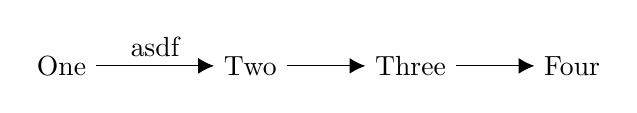
\begin{tikzpicture}
            \node[left] (one) { One };
            \draw[\standardarrow] (one.east) -- ++(1.5,0)  node[above, pos=0.5] { asdf }
            node[right] (two) { Two };
            \draw[\standardarrow] (two.east) -- ++(\standardlength)
            node[right] (three) { Three };
            \draw[\standardarrow] (three.east) -- ++(\standardlength)
            node[right] (four) { Four };
        \end{tikzpicture}
        \caption{ cap }
        \label{fig:two}
    \end{figure}

    \begin{figure}
        \centering
        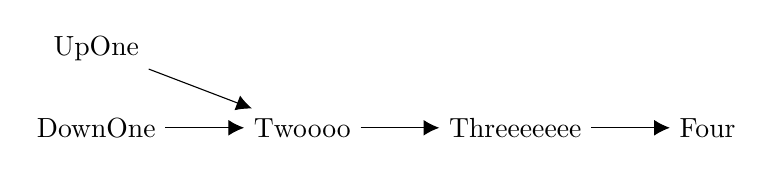
\begin{tikzpicture}
            \node (one) { UpOne };
            \node[below of=one] (two) { DownOne };
            \draw[\standardarrow] (two.east) -- ++(\standardlength)
            node[right] (three) { Twoooo };
            \draw[\standardarrow] (one) -- (three);
            \draw[\standardarrow] (three.east) -- ++(\standardlength)
            node[right] (four) { Threeeeeee };
            \draw[\standardarrow] (four.east) -- ++(\standardlength)
            node[right] (five) { Four };
        \end{tikzpicture}
        \caption{ cap }
        \label{fig:three}
    \end{figure}


\end{document}